%=========================================================================
% sec-xpc
%=========================================================================

\section{Thesis Proposal: Explicit-Parallel-Call Architectures}
\label{sec-xpc}

\begin{figure}[t]
  \begin{minipage}[b]{0.42\tw}
    %=========================================================================
% fig-intro-overview
%=========================================================================

%\begin{figure}

  \centering
  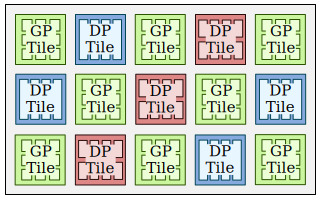
\includegraphics[width=0.85\tw]{intro-overview.svg.pdf}

  \caption{\textbf{Example of Fine-Grain Heterogeneous Architectures --}
    A sea of lightweight compute tiles composed of both general-purpose
    tiles (GP tiles) and data-parallel accelerators specialized for
    exploiting different forms of data parallelism (DP tiles).}

  \label{fig-intro-overview}

%\end{figure}

  \end{minipage}%
  \hfill%
  \begin{minipage}[b]{0.56\tw}
    %=========================================================================
% fig-intro-vision
%=========================================================================

%\begin{figure}

  \centering
  \includegraphics[width=\tw]{intro-vision.svg.pdf}

  \caption{\textbf{XPC Architecture Overview --} XPC applications use an
    XPC parallel programming library to expose fine-grain parallel tasks.
    A software runtime is used to facilitate adaptive task distribution
    across XPC tiles based on statistics collected during profiling. The
    heterogeneous XPC tiles are specialized for various forms of
    parallelism, but all XPC tiles have a common ISA.}

  \label{fig-intro-vision}

%\end{figure}

  \end{minipage}
\end{figure}

%In order to \emph{expose} fine-grain parallel tasks, we propose a
%parallel programming library coupled with a unified XPC instruction set
%architecture (ISA). To \emph{execute} parallel tasks, we propose a
%heterogeneous mix of microarchitectural tiles specialized for
%conventional and amorphous data parallelism. Finally, to \emph{schedule}
%parallel tasks, we propose a software runtime with hardware support for
%adaptive migration of tasks.

\subsection{Exposing Fine-Grain Parallel Tasks}

%\textbf{Exposing Parallel Tasks --}
The XPC programming framework exposes parallelism at a fine granularity
and provides support for nested parallelism. The framework enables
application developers to focus on exploring different algorithms for
implementing a given application (e.g., recursive, iterative, etc.) and
evaluating the tradeoffs of mapping different algorithms to different XPC
tiles. Several parallel primitives in the spirit of the Intel
TBB~\cite{reinders-tbb-book2007} library including \TT{parallel\_invoke}
for recursively generating tasks as well as \TT{parallel\_for} for
parallelizing loop iterations are provided.
%We take advantage of modern C++11 lambda functions to achieve a clean and
%convenient method for defining tasks.

The XPC ISA extends a traditional RISC ISA with three new instructions: a
parallel function call instruction (\TT{pcall}), a parallel function
return instruction (\TT{pret}), and a parallel synchronization
instruction (\TT{psync}). A parallel function call enables the software
to inform the hardware that it is acceptable to execute the callee in
parallel with the caller, but critically, parallel execution is \emph{not
  required}. \TT{pcall}s can be nested to arbitrary depths, and recursive
\TT{pcall}s are also allowed.  A \TT{pret} returns from a \TT{pcall} and
also acts as an implicit synchronization point. A particularly novel
feature of the XPC ISA is the ability to encode a parallel multi-call
which informs the hardware that the given function should be executed $n$
times where $n$ can be either specified at compile time or run time.

%While it is certainly possible to achieve the same effect by using a
%basic \TT{pcall} within a loop, a parallel multi-call enables very
%efficient execution on data-parallel accelerator tiles.

\subsection{Executing Fine-Grain Parallel Tasks}

%The underlying XPC microarchitecture is a heterogeneous mix of XPC tiles
%that are specialized for exploiting a broad range of amorphous data
%parallelism.

%\textbf{Executing Parallel Tasks --}
\textbf{XPC TCL Tile --} An XPC tile with tightly coupled lanes (TCL) is
a data-parallel accelerator specialized for regular data-parallelism. A
simple in-order, single-issue control processor manages an array of
lanes. Instruction fetch and decode are amortized by the control
processor and an issue unit schedules a group of threads to execute in
lock-step on the tightly coupled lanes.
%Control irregularity can cause divergence between threads, serializing
%execution of both paths of the branch. Memory accesses are dynamically
%coalesced by a memory unit by comparing the addresses generated across
%the lanes.
%Unlike GPGPUs, the TCL tile focuses on exploiting intra-warp parallelism
%instead of relying on extreme temporal multithreading to exploit
%inter-warp parallelism.
The TCL tile is inspired by my previous work on accelerating
regular data-parallel applications on GPGPUs by exploiting value
structure~\cite{kim-simt-vstruct-isca2013}.
%Similar techniques can be used to eliminate redundant computation.

%Although the TCL tile will achieve high performance and energy efficiency
%by amortizing the front-end and memory accesses as well as exploiting
%value structure for conventional data parallel tasks, it will struggle
%with the serialization caused by control and memory-access irregularity
%in amorphous data parallel tasks.

\textbf{XPC LCL Tile --} An XPC tile with loosely coupled lanes (LCL) is
an accelerator specialized for more irregular irregular data-parallelism.
The key difference between a TCL and an LCL tile is that an LCL tile
allows the control flow between lanes to be decoupled. This is achieved
by using per-lane instruction buffers that are pre-populated by the
control processor. The control processor still amortizes instruction
fetch and a lane management unit distributes tasks across the lanes. Each
LCL lane is more lightweight than its TCL counterpart since expensive
long-latency functional units and memory ports are shared across all
lanes and the control processor.
%As a result, LCL tiles will likely include more lanes than TCL tiles for
%roughly the same area.
The LCL design is inspired by previous work in our research group on
architectural specialization for inter-iteration loop dependence
patterns~\cite{srinath-xloops-micro2014}.

% The LCL tile can be used as reasonable middle-ground for accelerating
% amorphous data parallelism before resorting to a general-purpose tile
% because of its higher tolerance for control irregularity. However, the
% LCL tile is still better suited for simpler tasks on the lanes and can
% suffer from high memory-access irregularity.

\textbf{XPC CMC Tile --} An XPC tile with co-operative multicores (CMC)
can be used for highly irregular irregular data-parallel applications
that cannot be efficiently accelerated on other XPC tiles. A CMC tile
includes an array of discrete cores connected by a crossbar to facilitate
rapid inter-core communication and includes hardware acceleration for
scheduling fine-grain parallel tasks. The CMC tile can function as a
default tile for the profiling phase when statistics are collected to
determine if the application would be more suitable for a TCL or an LCL
tile.

% in addition to being the optimal tile for highly irregular amorphous
% data parallel tasks which cannot fully utilize the more structured TCL
% or LCL tiles.

% Each CMC core, albeit relatively simple, is akin to a stripped-down
% control processor in a TCL/LCL tile, making it capable of handling high
% control and memory-access irregularity with acceptable performance. The
% tradeoff is that CMC is the least energy efficient tile of the three
% XPC tiles for applications which exhibit more regular amorphous data
% parallelism. The key difference between the CMC tile and a traditional
% multicore is that

\subsection{Scheduling Fine-Grain Parallel Tasks}

%\begin{figure}
%  \begin{minipage}[b]{0.53\tw}
%    %=========================================================================
% fig-xpc-task-cache.tex
%=========================================================================

%\begin{figure}

  \centering
  \includegraphics[width=\tw]{task-cache.svg.pdf}

  \caption{\textbf{Task Cache Diagram --} Per-core task caches store
    generated tasks in hardware as a triplet of a function pointer, a
    stack pointer, and the number of calls for the task.}

  \label{fig-xpc-task-cache}

%\end{figure}


%  \end{minipage}%
%  \hfill%
%  \begin{minipage}[b]{0.45\tw}
%    %=========================================================================
% fig-xpc-task-network.tex
%=========================================================================

%\begin{figure}

  \centering
  \includegraphics[width=\tw]{task-network.svg.pdf}

  \caption{\textbf{Task Distribution Network Diagram --} Network
    connecting task caches for rapid distribution of tasks across
    heterogeneous XPC tiles based on meta-data describing task affinity
    with given tile.}

  \label{fig-xpc-task-network}

%\end{figure}


%  \end{minipage}
%\end{figure}

%The fine-grain parallel tasks exposed in software are mapped to the XPC
%tiles in hardware through a software runtime that adaptively schedules
%tasks onto the best suited tiles. This process can be accelerated in
%hardware with a \emph{task cache} and \emph{task distribution network}.

%\textbf{Scheduling Parallel Tasks --}
One way for the software runtime to manage parallel tasks is with
per-thread task queues in memory similar to the Intel TBB runtime
implementation~\cite{reinders-tbb-book2007}.
%Entries in the task queues are composed of a function pointer to the task
%available for parallel execution, as well as the thread ID of the parent
%that spawned this parallel task. A convenient consequence of using
%lambdas is that the arguments and local variables normally allocated on
%the stack are naturally captured to create a closure. This library-based
%approach is similar in spirit to the Intel TBB runtime
%implementation~\cite{reinders-tbb-book2007}. Idle threads can steal tasks
%by dequeuing tasks from the top of another thread's task queue, but a
%thread may always execute any tasks from its own task queue by dequeueing
%from the bottom.
I plan to explore techniques to bias the work stealing algorithm such
that tasks naturally migrate to the most appropriate XPC tile. The
runtime can collect statistics on control and memory-access irregularity
as proxies for performance and energy efficiency.
%Higher irregularity would suggest the task is better suited for more
%general-purpose tiles, whereas highly regular tasks would be better
%suited for data-parallel accelerator tiles.
Although the runtime normally generates and distributes tasks through
memory, hardware acceleration can be used to streamline these
processes. For example, a per-tile \emph{task cache} that exploits
intra-tile task locality can be used to store entries of the task queue.
%in a hardware cache to avoid memory accesses. This is based on the
%observation that each thread or tile will almost always need to access
%its own task queue whenever it is ready to execute a new
%task.
Furthermore, a \emph{task distribution network} can be used to
connect task caches in order to facilitate efficient task stealing
between tiles.
%The runtime triggers a broadcast of task steal requests if the tile it is
%running on is idle.
%For scalability, the request is only broadcasted to the tile's direct
%neighbors.
The network also communicates meta-data with each request describing the
type of task for which it is best suited, which can considered along with
collected statistics to determine whether or not a tile should allow task
stealing. These hardware techniques for storing and distributing tasks is
inspired by my previous work in task distribution for irregular
data-parallel applications on GPGPUs~\cite{kim-hwwl-micro2014}.  Similar
approaches to task distribution in traditional multicore systems have
been proposed~\cite{kumar-carbon-isca2007,sanchez-adm-asplos2010}, but
these techniques do not address heterogeneous architectures where a new
dimension of using heuristics to optimally schedule tasks across
different microarchitectural tiles must be considered.
